\documentclass[12pt]{article}
\usepackage[english]{babel}
\usepackage[utf8x]{inputenc}
\usepackage{amsmath}
\usepackage{graphicx}
\usepackage{blindtext}
\usepackage[colorinlistoftodos]{todonotes}
\usepackage{listings}
\usepackage{color} 
\definecolor{mygreen}{RGB}{28,172,0} 
\definecolor{mylilas}{RGB}{170,55,241}

\begin{document}

\begin{titlepage}

\newcommand{\HRule}{\rule{\linewidth}{0.5mm}} 
\center 
 

%	HEADING SECTIONS
\title{Práctica 1}
\textsc{\LARGE Instituto Tecnológico de Morelia}\\[1.1cm]
\textsc{\Large Práctica 1}\\[0.3cm]
\textsc{\large Control 1}\\[0.3cm] 
%	TITLE SECTION

\HRule \\[0.4cm]
{ \huge \bfseries Análisis de un Sistema de Primer Orden}\\[0.2cm] 
\HRule \\[1cm]

%	AUTHOR SECTION
\begin{minipage}{0.5\textwidth}
\begin{flushleft} \large
\emph{Autor[1]:}\\
José Raymundo \textsc{Santana Ruiz} \\
\emph{Autor[2]:}\\
Irving \textsc{Arroyo Reyes}
\end{flushleft}
\end{minipage}
~
\begin{minipage}{0.4\textwidth}
\begin{flushright} \large
\emph{Supervisor:} \\
Gerardo Marx \textsc{Chaves Campos} 
\end{flushright}
\end{minipage}\\[1cm]
{\large \today}\\[1cm]

\includegraphics[width=2.5in]{Itmorelia.png}\\[1cm] 
\vfill % Fill the rest of the page with whitespace
\end{titlepage}

\section{Introducción}

Un sistema de primer orden está caracterizado por tener solamente un elemento capaz de almacenar energía y por lo tanto estarán estos sistemas caracterizados por ecuaciones diferenciales ordinarias de primer orden.\\

Los sistemas de primer orden, pueden en general ser de tipo:
\begin{itemize}
\item Eléctrico
\item Mectánico
\item Hidráulico
\item Térmico
\item Híbridos
\end{itemize}

Cabe señalar que se pueden obtener modelos matemáticos para todas las variables que interfieren en los sitemas a modelar. Las leyes básicas que controlan los circuitos eléctricos son las leyes de Kirchhoff, para sistemas mecánicos la segunda ley de Newton y así cada sistema de control de primer orden tiene sus leyes básicas que rigen su comportamiento.

Por lo tanto existen muchas variantes de los mismos.\\

Sin embargo, para convenciencia, los análisis de estos sitemas son hechos de manera que se parta de modelos genéricos que representen a los sistemas a analizar.\\

Tal modelo tendrá la siguiente estructura:

\begin{equation}
a_0\frac{dy(t)}{dt}+a_1y(t)=b_0u'(t)+b_1u(t)
\end{equation}



\subsection{Respuesta al Impulso de Sistemas de Primer Orden}

En este caso, la respuesta se obtiene cuando el sistema se ve excitado por una función impulso y además se considera que el sistema no tiene energía almacenada, lo que significa que su condición inicial es cero.\\

Una forma de desarrollar la idea es mediante la transformada de Laplace, lo que significará que la respuesta del sistema crecerá (o decrecerá), comenzando desde el origen hasta llegar a un límite.\\

Este tipo de respuesta tomará un tiempo definido para completarse, y éste viene determinado por el sistema.
La respuesta del sistema nos da una relación con la función de transferencia, la cual es la representación más general que pueden tener los sistemas lineales e invariantes en el tiempo.\\

Para esta práctica consideraremos la función de transferencia general como la siguiente:

\begin{equation}
H(s)=\frac{bs+c}{s+a} \label{eq:2}
\end{equation}

\section{Metodología}
\subsection{Experimento 1}

Para la primera sección del experimento, tendremos que resolver la ecuación \eqref{eq:2} para que mediante la implementación de un código de Scilab, éste sea capaz de entregarnos una gráfica con la respuesta del sistema siguiente:\\

\begin{center}
    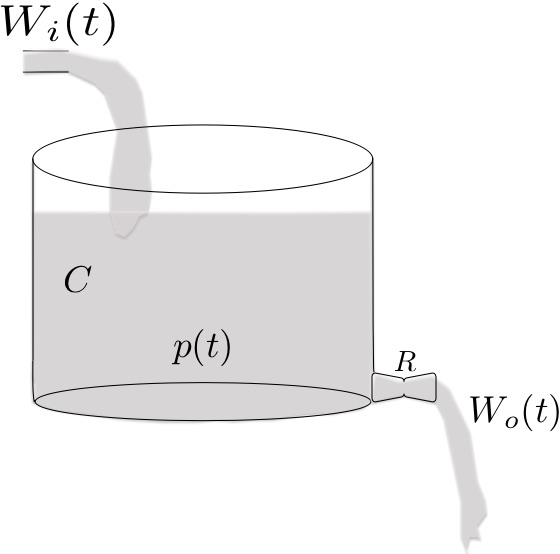
\includegraphics[width=2.3in]{tankScheme.jpg}
    \begin{figure}[!h]
	\caption{Figura del Ejercicio.}\label{ref:FiguraA}
	\end{figure}
\end{center}

Como se aprecia en la ecuación \eqref{eq:2}, ésta tiene los coeficientes a, b y c que se relacionan a propiedades del sistema, lo que se requiere hacer es que el código de matlab, implementado valores para tales coeficientes, debrá ser capaz de resolver la ecuación.\\

Para hacerlo se deberá reescribir la ecuación \eqref{eq:2} como sigue:

\begin{equation}
Y(s)=\frac{A}{s}+\frac{B}{s+a} \label{eq:3}
\end{equation}

El equipo de trabajo entonces deberá resolver tal expresión para obtener una respuesta genérica que se implementará con casos generales donde:

\begin{enumerate}
\item El flujo de entrada es mayor que el de salida.
\item El flujo de salida es mayor que el de entrada.
\item Ambos flujos son iguales.
\end{enumerate}

Se deberá añadir las gráficas de tales respuestas.

\subsection{Resolución del Problema}

Partiendo de la ecuación \eqref{eq:2}, pasaremos a una forma similar a como se ve la ecuación \eqref{eq:3}.\\

Para resolver ambas ecuaciones debemos igualarlas y obtendremos algo similar a:

\begin{equation}
	\frac{bs+c}{s+a} = \frac{A}{s}+\frac{B}{s+a}
\end{equation}

De ahí despejaremos el numerado de la parte izquierda y obtendremos la expresión:

\begin{equation}
	bs + c = \left(\frac{A}{s}+\frac{B}{s+a}\right) * (s+a)
\end{equation}

Resolviendo entonces para el coeficiente A, obtendremos que su valor está dado por la relación:

\begin{equation}
	A = \frac{c}{a}
\end{equation}

Y a su vez, el coeficiente B, está dado por el valor:

\begin{equation}
	B = \frac{ab-c}{a}
\end{equation}

Una vez obtenidos tales valores, debemos transformar las expresiones de fracciones parciales a una expresión determinada por la función impulso, esto se hace mediante la transformada de Laplace.\\

Tal expresión quedará de la siguiente manera:

\begin{equation}
	Y(t) = A(Us(t)) + B(e^{-at}*Us(t))
\end{equation}

Factorizamos entonces el término del impulso y obtendremos la expresión final:

\begin{equation}
	H(t) = Us(t)\left[ A + Be^{-at} \right]
\end{equation}

Esta última ecuación es la que se implementa en el código de Scilab y queda de la siguiente manera.

\subsection{Implementación en Scilab}

El código de Scilab es el siguiente:

\lstset{language=Matlab,
    breaklines=true,
    morekeywords={matlab2tikz},
    keywordstyle=\color{blue},
    morekeywords=[2]{1}, keywordstyle=[2]{\color{black}},
    identifierstyle=\color{black},
    stringstyle=\color{mylilas},
    commentstyle=\color{mygreen},
    showstringspaces=false,
    numbers=left,
    numberstyle={\tiny \color{black}},
    numbersep=9pt, 
    emph=[1]{for,end,break},emphstyle=[1]\color{red}, 
}
\begin{lstlisting}[frame=single]    % super cooles Programm
	a=1;
	b=0;
	c=1;
	A= c/a;
	B= ((a*b)-c)/a;
	t=0:0.01:15;
	H=[A+(B*exp(-a*t))]
	plot(t,H)
\end{lstlisting}

Este programa entregará una gráfica que representa el comportamiento del sistema en el dominio del tiempo, mediante incrementos discretos de una variable de control del tiempo.\\

A su vez, se espera que el programa entregue un resultado similar al código presentado por el maestro que es el siguiente:

\lstset{language=Matlab,
    breaklines=true,
    morekeywords={matlab2tikz},
    keywordstyle=\color{blue},
    morekeywords=[2]{1}, keywordstyle=[2]{\color{black}},
    identifierstyle=\color{black},
    stringstyle=\color{mylilas},
    commentstyle=\color{mygreen},
    showstringspaces=false,
    numbers=left,
    numberstyle={\tiny \color{black}},
    numbersep=9pt, 
    emph=[1]{for,end,break},emphstyle=[1]\color{red},
}
\begin{lstlisting}[frame=single]    % super cooles Programm
	s = %s // la alternativa más rápida para s = ply (0,'s')
	// Ganancia y Constante de Tiempo
	k = 1;
	Tau = 1;
	simplesys = syslin('c', k/(1+Tau*s))
	t=0:0.01:15;
	y=csim('step',t,simplesys)
	plot(t,y)
\end{lstlisting}

\section{Resultados y discusiónes}

Las gráficas esperadas para las respuestas pedidas anteriormente son las siguientes:

\begin{center}
    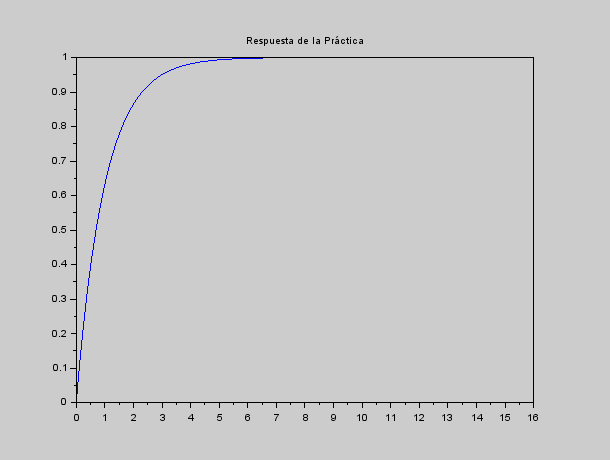
\includegraphics[width=2.5in]{SalidaMenor.png}
    \begin{figure}[!h]
	\caption{Gráfica de la respuesta cuando la salida es Menor.}\label{ref:Figura1}
	\end{figure}
\end{center}

En la figura \ref{ref:Figura1} podemos ver cómo es la respuesta del sistema cuando el flujo de salida es menor que el de entrada, también cabe aclarar que es prácticamente la misma gráfica que se genera al implementar el código de ejemplo del profesor.\\

Para el caso cuando el flujo de salida es mayor que el de entrada se genera la siguiente gráfica

\begin{center}
    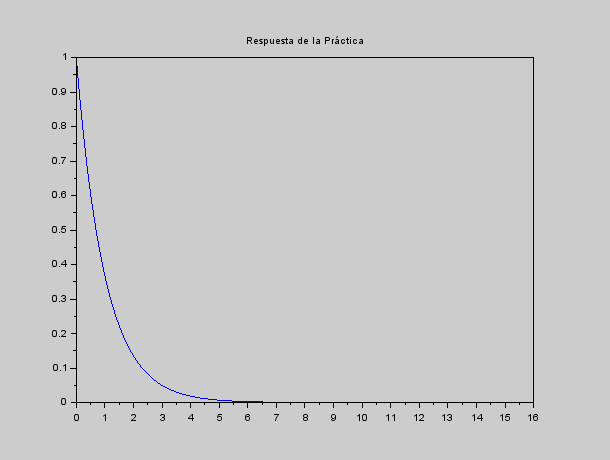
\includegraphics[width=2.5in]{SalidaMayor.png}
    \begin{figure}[!h]
	\caption{Gráfica de la respuesta cuando la salida es Mayor.}\label{ref:Figura2}
	\end{figure}
\end{center}

El comportamiento presentado en la figura \ref{ref:Figura2} es algo bastante lógico tomando en cuenta la gráfica previamente visualizada de la respuesta cuando el flujo de salida es menor que el de entrada.\\

Entonces sólo queda implementar la gráfica cuando el flujo de salida es igual que el de entrada, y eso nos generará una gráfica de que tiene la siguiente forma:

\begin{center}
    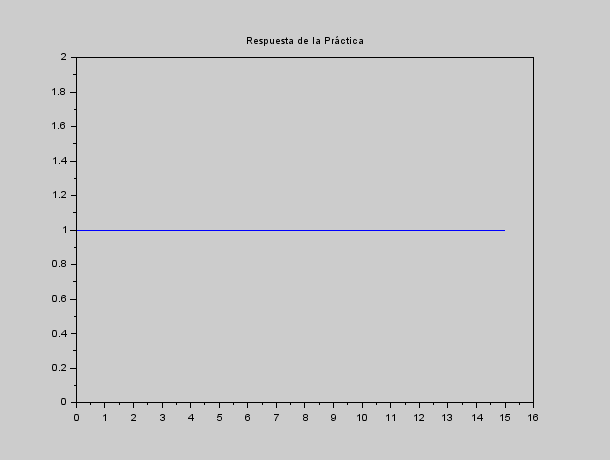
\includegraphics[width=2.5in]{SalidaIgual.png}
    \begin{figure}[!h]
	\caption{Gráfica de la respuesta cuando la salida es Igual.}\label{ref:Figura3}
	\end{figure}
\end{center}

Podemos observar que esta respuesta también es muy lógica considerando las previamente mostradas.

\section{Conclusiones}

El estudio de sistemas de primer orden se realiza a travéz del análisis de la respuestas de sus entradas, como lo son las funciones escalón e impulso. A partir de estas respuestas (escalón e impulso) se pueden conocer las características del sistema y poder observar las formas de onda estándar.

Para obtener la función de transferencia de un sistema de primer orden se ocupa sacar la transformada inversa de Laplace para esto las condiciones iniciales deben de ser cero (no hay energía almacenada en el sistema).


\section{Referencias}
1.- "Modern Control Sistem" Richard C. Dorf.

2.- "Ingeniería de control moderna" Katsuhiko Ogata.

3.-  https://prezi.com/ebxut275ww2f/sistemas-de-primer-orden/.


\end{document}
